\documentclass[11pt]{article}
\usepackage[utf8]{inputenc}
\usepackage{fancyhdr}
\usepackage[english]{babel}
\usepackage{graphicx}
\usepackage{array}
\usepackage{amsmath}
\usepackage{amssymb}
\usepackage{mathtools}
\usepackage{algorithmicx}
\usepackage{algpseudocode}
\renewcommand{\baselinestretch}{1.0}
\usepackage[letterpaper, margin=0.75in]{geometry}
\DeclarePairedDelimiter{\ceil}{\lceil}{\rceil}
\pagestyle{fancy}
\lhead{}
\rhead{Yu Mi, yxm319. Algorithm HW1}
\begin{document}
	\title{Homework2 for EECS 340}
	\author{Yu Mi,yxm319}
	\maketitle
\section{Give a recursive algorithm to find the average (mean) value of an array of $2^k$ decimal numbers, where $k\in \mathbb{N}$.}
	\emph{Answer:} The proposed algorithm is as follow:
	
	\begin{algorithmic}
	\State \textbf{Algorithm A1}: Average($L$)
	\State \textbf{Data}: A list of $2^k$ decimal numbers $L$.
	\State \textbf{Result}: The average of all the numbers in $L$.
	\If {$L$.length()$=0$} 
		\State \Return $L[0]$
	\Else
		\State $length\gets L.length()$
		\State \Return $0.5\times$$($Average($L[0,length/2-1]+$Average($L[length/2,length]$)$)$
	\EndIf
	\end{algorithmic}
\section{R-12.6}
	\emph{Question}:Suppose we are given a set of telescope observation requests, specified by triples, of $(s_i, f_i, b_i)$, defining the start times, finish times, and benefits of each observation request as
	\begin{equation*}
		L={(1,2,5),(1,3,4),(2,4,7), (3,5,2), (1,6,3), (4,7,5), (6,8,7), (7,9,4)}
	\end{equation*}
	Solve the telescope scheduling problem for this set of observation requests.
	
\noindent	\emph{Answer}: The time of scheduling can be shown in Fig.\ref{fig:fig1}, the number in the bar means the value of such task. 
	\begin{figure}[h]
		\centering
		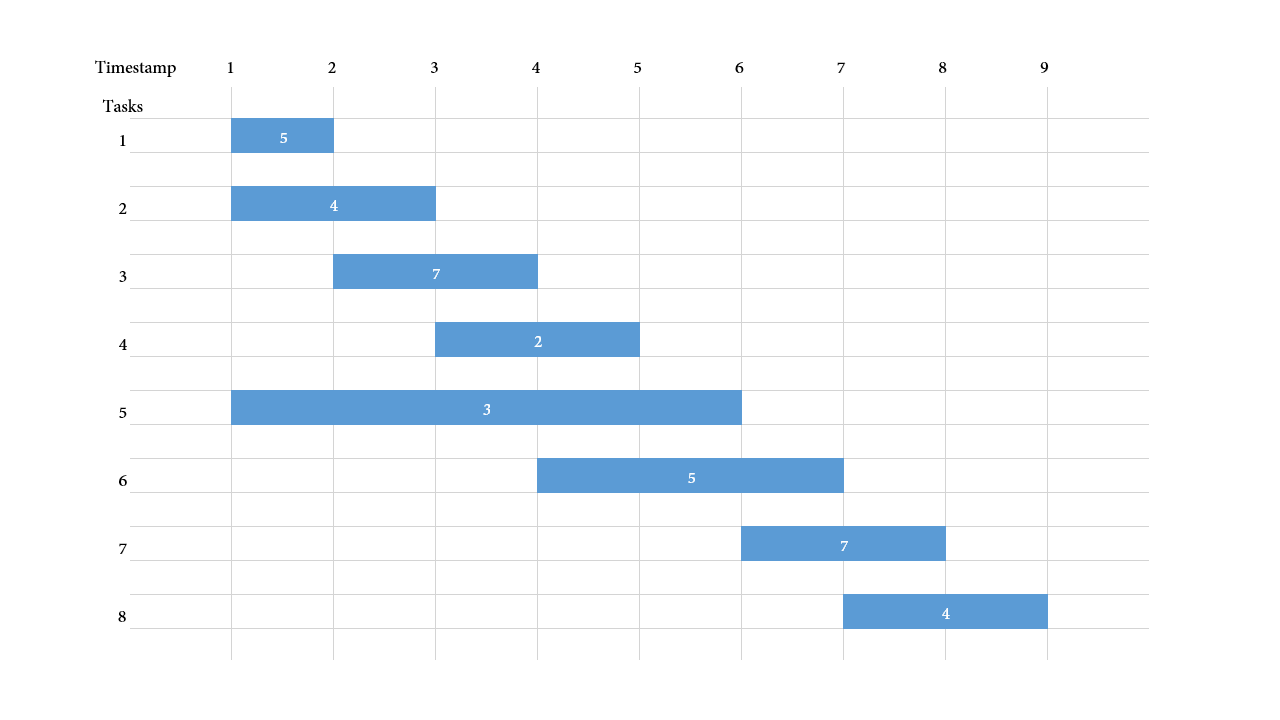
\includegraphics[width=0.62\textwidth]{Figure/FG1.png}
		\caption{Time of tasks}
		\label{fig:fig1}
	\end{figure}
	
	Based on what we have discussed on class, we can have a table of $B_i$ which stands for the maximum benefit that can be achieved with the first $i$ requests in the task list. 
	
	To fill this table, we follow the algorithm as follow:
	\begin{algorithmic}
	\State $B[0]\gets0$
	\For {$i$ = 1 to $n$ }
	\State     $B[i]\gets max(B[i-1],B[P[i]]+b_i)$
	\EndFor
	\end{algorithmic}
	
	Here the $P[i]$ stands for the array which gives the predecessor index for each request $i$, and $b_i$ means the value of each single task. The table is shown as Table \ref{tab:tab1}.
	\begin{table}[!hbp]
		\centering
		\caption{$B_i$ values}
			\begin{tabular}{c|c|c|c|c|c|c|c|c|c}
			\hline 
			\hline
			$i$  &$0 $& $1$ & $2$& $3$& $4$& $5$& $6$& $7$& $8$\\
			\hline
			$B_i$& 0  & 5   & 4  & 12 & 6  & 3  & 17 & 13 &21\\
			\hline
			\hline
			\end{tabular}
		\label{tab:tab1}
	\end{table}
	
	As we can see, the highest value is $B_8$, which includes task $1,3,6,8$ that we should select. The corresponding triples are $(1,2,5), (2,4,7),(4,7,5),(7,9,4)$.
\section{Implement \emph{det-bogoSort} in pseudocode using recursion}
\end{document}